% FaCTS — Review 3 reference paper (AI-assisted draft for the team).
% Build:  tectonic main.tex        (or upload this folder to Overleaf)
% Every number in tables/*.tex is generated by scripts/make_paper_tables.py from reports/eval_review3/;
% numbers written in the text were copied from those tables. Re-run the script after any new evaluation.
\documentclass[conference]{IEEEtran}
\IEEEoverridecommandlockouts
\usepackage{cite}
\usepackage{amsmath,amssymb,amsfonts}
\usepackage{algorithm}
\usepackage{algpseudocode}
\usepackage{graphicx}
\usepackage{booktabs}
\usepackage{multirow}
\usepackage{array}
\usepackage{xcolor}
\usepackage{tikz}
\usetikzlibrary{arrows.meta,positioning,fit,calc}
\usepackage[hidelinks]{hyperref}
\newcommand{\draftnote}[1]{\textcolor{red!70!black}{\textbf{[#1]}}}

\begin{document}

\title{FaCTS: Fact-Conditioned Generation and Sentence-Level Verification for Faithful Clinical Note Generation from Doctor--Patient Conversations}

\author{\IEEEauthorblockN{V. Hirthick Srinivaasan, Keerthana Saravanan, Ruchitha Reddy}
\IEEEauthorblockA{School of Computer Science and Engineering, VIT Chennai, India\\
24BRS1281, 24BRS1140, 24BRS1259}
\thanks{\textbf{Reference draft for the team (AI-assisted).} It shows the structure, content and evidence the
Review~3 paper needs. Rewrite it in your own words before submission. Every experimental number is
reproducible from the repository (\texttt{reports/eval\_review3/}).}}

\maketitle

% =====================================================================================================
\begin{abstract}
Large language models (LLMs) can draft clinical notes from doctor--patient conversations, but a fluent
note may contain symptoms, medications or doses that were never said. We study this problem on two public
benchmarks, ACI-Bench (full visit notes) and MTS-Dialog (note sections), and propose FaCTS, a pipeline that
(i) extracts clinical facts with negation and dosage attributes from the transcript, (ii) conditions an
open 8B LLM (Llama-3.1-8B-Instruct, 4-bit) on a fact table, and (iii) checks every generated sentence
against the best-matching transcript turns with a BM25 retriever and a DeBERTa-v3 natural-language-inference
verifier, dropping unsupported sentences. A plain QLoRA fine-tuned baseline is trained for comparison.
% Numbers from reports/eval_review3/summary.md and research_paper/published_results.md.
On ACI-Bench test~1 the untrained model reaches ROUGE-1 0.519, equal to GPT-4 zero-shot (0.518) in the
MEDIQA-Chat 2023 shared task, against 0.614 for the best GPT-4 in-context system; on MTS-Dialog the
fine-tuned model reaches 0.400, level with fine-tuned shared-task systems (0.395--0.401). However, QLoRA
fine-tuning raised the entity-level hallucination rate from 14.4\% to 51.7\% (ACI-Bench) and from 20.4\% to
35.6\% (MTS-Dialog); giving the fine-tuned model the fact table did not undo this. The fact table lowered hallucination to 10.6\% and 15.8\% without loss of coverage, giving
the best fact-level F1 (82.8 and 77.4); verification lowered it further to 8.7\% and 14.2\% at a cost in
coverage.

\end{abstract}

\begin{IEEEkeywords}
Clinical note generation, hallucination, large language models, QLoRA, natural language inference,
factual consistency, doctor--patient dialogue summarization.
\end{IEEEkeywords}

% =====================================================================================================
\section{Introduction}

\subsection{Problem domain}
Clinicians spend a large share of their working time on documentation; physicians can spend up to two
hours on the electronic health record for every hour of direct patient care~\cite{vanveen2024}.
Automatically drafting the visit note from the recorded consultation --- \emph{ambient clinical
documentation} --- is therefore one of the most requested applications of LLMs in
healthcare~\cite{asgari2025,yim2023aci}. Public benchmarks for the task now exist: ACI-Bench pairs full
doctor--patient encounters with complete visit notes~\cite{yim2023aci}, and MTS-Dialog pairs shorter
conversations with individual note sections~\cite{abacha2023mts}. The MEDIQA-Chat 2023 shared task used
both and showed that LLM-based systems reach the highest automatic scores~\cite{abacha2023overview}.

\subsection{Problem statement}
High ROUGE or BERTScore does not mean that a note is safe. A clinical note is a legal and medical record:
a single invented allergy, a flipped negation (``denies chest pain'' $\rightarrow$ ``reports chest pain'')
or a changed dose can lead to a wrong treatment decision~\cite{asgari2025}. LLMs produce such
\emph{hallucinations} --- content not supported by the source --- even when the text reads
fluently~\cite{bn2025fact,das2025}, and general-domain hallucination detectors transfer poorly to clinical
dialogue~\cite{bn2025fact}. A second, less discussed problem concerns how open models are adapted:
supervised fine-tuning (SFT) on targets that contain information not present in the input has been shown to
increase hallucination in general-domain LLMs~\cite{gekhman2024,kaplan2026}. Clinical reference notes
contain exactly such information (content the clinician knew but did not say aloud), so standard
fine-tuning may teach a model to write plausible but ungrounded details.

Formally, given a de-identified transcript $D$ of a completed outpatient consultation, the system must
produce a structured note $\hat{y}$ (a full note for ACI-Bench, one requested section for MTS-Dialog) such
that every clinical statement in $\hat{y}$ is supported by $D$, while covering the clinically important
facts of the reference note $y$. Speech recognition, live deployment and EHR integration are out of scope.

\subsection{Existing approaches}
Systems in the literature fall into three groups: (a) fine-tuned encoder--decoder models such as BART and
LongT5~\cite{sharma2023cadence,abacha2023mts}; (b) in-context learning with large proprietary models such as
GPT-4~\cite{giorgi2023wanglab,abacha2023overview}; and (c) parameter-efficient adaptation of open LLMs with
QLoRA or prompt tuning~\cite{vanveen2024,lyu2024}. Most report lexical overlap only; factuality is either
not measured or measured by human review on small samples~\cite{giorgi2023wanglab,vanveen2024}.

\subsection{Proposed idea}
Instead of trusting the generator, FaCTS constrains it from both sides. Before generation, a deterministic
clinical fact extractor turns the transcript into a fact table (entity, category, negation status, dose)
that is placed in the prompt. After generation, each sentence is verified against the transcript by an
NLI model and unsupported sentences are removed. Both stages work with any generator and need no GPU
training.

\subsection{Contributions}
\begin{itemize}
\item A reproducible evaluation of an open 8B LLM on the official ACI-Bench and MTS-Dialog test sets,
  compared with the published MEDIQA-Chat 2023 systems using the official ROUGE configuration.
\item Evidence that plain QLoRA fine-tuning raises the entity-level hallucination rate compared with the
  same model used zero-shot, consistent with findings on fine-tuning and new knowledge~\cite{gekhman2024}.
\item FaCTS: a fact-conditioned prompt built from a negation-aware clinical fact extractor, and a
  sentence-level BM25\,+\,NLI verifier with flag-and-drop, evaluated as an ablation (zero-shot $\rightarrow$
  +fact table $\rightarrow$ +verifier).
\item A clinical factuality evaluation that reports hallucination, negation-flip, numerical consistency and
  coverage, and maps them to fact-level precision, recall and F1.
\end{itemize}

\subsection{Organisation}
Section~\ref{sec:lit} reviews fifteen related papers and states the research gap.
Section~\ref{sec:method} describes the proposed system, the LLM architecture, the equations and the
algorithm. Section~\ref{sec:exp} presents the datasets, tools, metrics and results on each dataset, with
comparison to published results. Section~\ref{sec:conc} concludes and outlines future work.

% =====================================================================================================
\section{Literature Survey}\label{sec:lit}

\subsection{Papers explaining the problem}
\textbf{Asgari et al.}~\cite{asgari2025} propose CREOLA, a clinician-in-the-loop framework with an error
taxonomy and a clinical-safety grading for LLM-generated notes. Over 18 experimental configurations and
12,999 clinician-annotated sentences they measure a 1.47\% hallucination rate and a 3.45\% omission rate,
and show that prompt and workflow changes can push major errors below reported human error rates. The
work establishes that hallucinations and omissions must be measured separately and graded by harm.

\textbf{BN et al.}~\cite{bn2025fact} study hallucinations in summaries of patient--clinician dialogues.
They build a fact-controlled ``leave-N-out'' dataset by deleting facts from source dialogues, and a set of
natural hallucinations, and find that general-domain detectors fail on clinical hallucinations and that
performance on synthetic hallucinations does not predict performance on natural ones; fact-counting
detectors give explainable scores.

\textbf{Das et al.}~\cite{das2025} evaluate open-source LLMs (e.g., Qwen2.5, DeepSeek-v2) on extracting key
events from discharge summaries and categorise the hallucinations they produce. The models capture
admission reasons well but are inconsistent on follow-up recommendations, showing that errors concentrate
in specific clinical content types.

\textbf{Gekhman et al.}~\cite{gekhman2024} show in a controlled study that fine-tuning examples which
introduce knowledge new to the model are learned slowly, and that once learned they linearly increase the
model's tendency to hallucinate. \textbf{Kaplan et al.}~\cite{kaplan2026} confirm that exposure to new
facts through SFT increases hallucination with respect to pre-trained knowledge, trace it to interference
between overlapping representations, and mitigate it with self-distillation or parameter freezing. Both are
general-domain studies; they explain why fine-tuning on clinical notes that contain unspoken information
can raise hallucination.

\subsection{Papers on existing approaches}
\textbf{Ben Abacha et al.}~\cite{abacha2023overview} organised MEDIQA-Chat 2023: Task~A summarises
MTS-Dialog conversations into note sections (1,201/100/200 train/validation/test) and Task~B generates full
ACI-Bench notes (67/20/40). Short notes were ranked by the mean of ROUGE-1, BERTScore and BLEURT, full
notes by ROUGE-1; GPT-4 in-context learning ranked first in both tasks.

\textbf{Giorgi et al. (WangLab)}~\cite{giorgi2023wanglab} compare fine-tuning a Longformer
encoder--decoder with few-shot in-context learning of GPT-4 using retrieved similar examples; the ICL system
ranked first (ROUGE-1 0.614 on ACI-Bench test~1), and physicians preferred its notes about as often as the
human-written ones.

\textbf{Sharma et al. (Cadence)}~\cite{sharma2023cadence} take a data-augmentation-first approach: a
BART model generates synthetic dialogues from MIMIC-IV notes (Task~C), which are added to the training data
of BART summarisers with an N-pass strategy for long inputs; theirs were the only stable and reproducible
runs on all three tasks.

\textbf{Van Veen et al.}~\cite{vanveen2024} adapt eight LLMs with in-context learning and QLoRA across four
clinical summarisation tasks, including doctor--patient dialogue (ACI-Bench). In a reader study with ten
physicians, summaries of the best adapted model were non-inferior to human summaries in 45\% of cases and
preferred in 36\%; they also report fabricated content in both LLM and human summaries.

\textbf{Lyu et al.}~\cite{lyu2024} apply soft prompt tuning to GatorTronGPT (5B and 20B) on MTS-Dialog.
The 20B model with 302M trainable parameters reached ROUGE-1 0.363 on the 400-item test set, above a fully
fine-tuned T5-Large (0.343), showing that parameter-efficient adaptation of large decoders is competitive.

\subsection{Papers related to our methodology}
\textbf{Dettmers et al.}~\cite{dettmers2023qlora} introduce QLoRA: back-propagation through a frozen
4-bit NormalFloat (NF4) model into low-rank adapters, with double quantisation and paged optimisers, which
matches 16-bit fine-tuning while fitting large models on one GPU. Our baseline uses QLoRA unchanged.

\textbf{Hu et al.}~\cite{hu2022lora} propose LoRA, which freezes pre-trained weights and learns a low-rank
update $\Delta W = BA$ in each adapted layer, cutting trainable parameters by orders of magnitude without
inference latency.

\textbf{Laban et al.}~\cite{laban2022summac} show that NLI models detect summary inconsistencies well when
applied at sentence level rather than document level (SummaC). Our verifier follows this idea, but retrieves
the relevant transcript turns first because a dialogue is too long and too noisy to serve as a premise.

\textbf{Huang et al. (SWING)}~\cite{huang2023swing} use NLI signals during training of dialogue summarisers
to increase coverage of reference content while penalising inconsistent sentences, demonstrating that NLI
judgements transfer to conversational input.

\textbf{Seethakantha et al.}~\cite{seethakantha2026hdsr} use hallucination detectors to guide iterative
revision of clinical summaries (HDSR) and turn the revision trajectories into preference pairs (HDSR-PL),
reducing hallucinations of Llama-3.1-8B-Instruct by 24\% and 48\% respectively on MIMIC-IV notes while
preserving fluency. In the same study, supervised fine-tuning on clinician-written references nearly doubled
the clinician-annotated hallucination count of Llama-3.1-8B-Instruct compared with zero-shot prompting
(57 vs.\ 29), the clinical counterpart of~\cite{gekhman2024}. Detector-guided repair and preference learning are the two directions our verifier and
our planned preference-tuning stage follow.

\subsection{Comparison and research gap}
Table~\ref{tab:lit} compares the fifteen papers. Three gaps emerge. (1) Systems on the public dialogue
benchmarks~\cite{abacha2023overview,giorgi2023wanglab,sharma2023cadence,lyu2024} report lexical metrics
only; factuality is measured either on proprietary data~\cite{asgari2025} or on other tasks such as
discharge summaries~\cite{das2025,seethakantha2026hdsr}. (2) Parameter-efficient fine-tuning is used as the
default way to adapt open models~\cite{vanveen2024,lyu2024}, although fine-tuning can increase hallucination
in general-domain QA~\cite{gekhman2024,kaplan2026} and in discharge-note summarisation~\cite{seethakantha2026hdsr};
this has not been measured on the public doctor--patient dialogue benchmarks. (3) NLI verification works at sentence level on news~\cite{laban2022summac} and
chit-chat dialogue~\cite{huang2023swing}, but clinical dialogues need evidence retrieval and negation
handling first. FaCTS addresses (1) by reporting entity-level factuality next to the official ROUGE on
ACI-Bench and MTS-Dialog, (2) by measuring zero-shot vs QLoRA hallucination on the same test sets, and (3) by
combining a negation-aware fact table with retrieval-then-NLI verification.

\begin{table*}[t]
\centering
\caption{Comparison of the surveyed papers}\label{tab:lit}
\footnotesize
\begin{tabular}{@{}p{2.6cm}p{0.6cm}p{2.5cm}p{3.5cm}p{3.3cm}p{3.4cm}@{}}
\toprule
Paper & Year & Data & Method & Key result & Limitation for our problem\\
\midrule
\multicolumn{6}{@{}l}{\emph{Problem}}\\
Asgari et al.~\cite{asgari2025} & 2025 & Proprietary consultations & CREOLA error taxonomy, clinician review & 1.47\% hallucination, 3.45\% omission (sentences) & Manual; not on public benchmarks\\
BN et al.~\cite{bn2025fact} & 2025 & Patient--clinician dialogue summaries & Fact-controlled leave-N-out hallucinations & General detectors fail on clinical text & Detection only, no mitigation\\
Das et al.~\cite{das2025} & 2025 & Discharge summaries & Open LLMs, key-event extraction & Follow-up actions least reliable & Discharge notes, not dialogue\\
Gekhman et al.~\cite{gekhman2024} & 2024 & Closed-book QA & Controlled fine-tuning on new knowledge & New knowledge raises hallucination linearly & General domain\\
Kaplan et al.~\cite{kaplan2026} & 2026 & QA, synthetic facts & Self-distillation SFT, freezing & Reduces SFT-induced hallucination & General domain\\
\midrule
\multicolumn{6}{@{}l}{\emph{Existing approaches}}\\
Ben Abacha et al.~\cite{abacha2023overview} & 2023 & MTS-Dialog, ACI-Bench & Shared task, 14 (A) and 9 (B) teams & GPT-4 ICL best & Lexical/semantic metrics only\\
Giorgi et al.~\cite{giorgi2023wanglab} & 2023 & ACI-Bench, MTS-Dialog & GPT-4 ICL vs fine-tuned LED & R-1 0.614 (ACI test 1) & Proprietary model; no factuality metric\\
Sharma et al.~\cite{sharma2023cadence} & 2023 & MTS-Dialog, ACI-Bench & BART + synthetic dialogues & Stable, reproducible runs & Small model; no factuality metric\\
Van Veen et al.~\cite{vanveen2024} & 2024 & 6 datasets incl.\ ACI-Bench & ICL vs QLoRA, 8 LLMs, reader study & LLM preferred/non-inferior in 81\% & A\&P section only for dialogue\\
Lyu et al.~\cite{lyu2024} & 2024 & MTS-Dialog & Soft prompt tuning, GatorTronGPT-20B & R-1 0.363 (400 test) & 20B model, 8$\times$A100; lexical only\\
\midrule
\multicolumn{6}{@{}l}{\emph{Methodology}}\\
Dettmers et al.~\cite{dettmers2023qlora} & 2023 & Instruction data & QLoRA: NF4, double quant., paged opt. & 16-bit quality on one GPU & No factuality control\\
Hu et al.~\cite{hu2022lora} & 2022 & GLUE, generation & Low-rank adapters & Large reduction in trainable params & No factuality control\\
Laban et al.~\cite{laban2022summac} & 2022 & SummaC benchmark (news) & Sentence-level NLI & Strong inconsistency detection & News, not dialogue\\
Huang et al.~\cite{huang2023swing} & 2023 & DialogSum, SAMSum & NLI-based training signals & Better coverage and faithfulness & Chit-chat, not clinical\\
Seethakantha et al.~\cite{seethakantha2026hdsr} & 2026 & MIMIC-IV notes & Detector-guided refinement + preference learning & $-$48\% hallucination; SFT doubles it (Llama-3.1-8B) & Notes, not dialogue; clinician labels needed\\
\bottomrule
\end{tabular}
\end{table*}

% =====================================================================================================
\section{Proposed Methodology}\label{sec:method}

\subsection{Technology}
FaCTS is implemented in Python with PyTorch, Hugging Face Transformers, PEFT and bitsandbytes for the LLM,
\texttt{rank-bm25} for retrieval and a DeBERTa-v3 cross-encoder for NLI. The generator is
Llama-3.1-8B-Instruct~\cite{dubey2024llama3} quantised to 4-bit NF4. Training and generation run on Kaggle
(2$\times$NVIDIA T4, 16\,GB each); fact extraction, verification and evaluation run on a laptop
(NVIDIA RTX~2050, 4\,GB).

\subsection{System architecture}
Fig.~\ref{fig:arch} shows the pipeline. It has four stages: (1) clinical fact extraction, (2) fact-table
construction and prompt building, (3) LLM generation, and (4) evidence retrieval, NLI verification and
filtering. The output is the clinical note, a verdict (green/yellow/red) for each sentence, and the ids
of the transcript turns that support it (provenance).

\begin{figure*}[t]
\centering
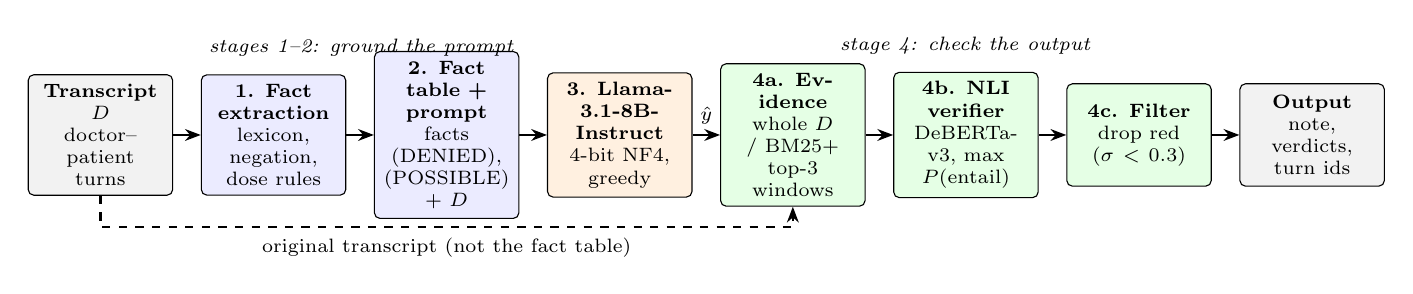
\begin{tikzpicture}[node distance=3.5mm, font=\scriptsize,
  box/.style={draw, rounded corners=2pt, align=center, minimum height=13mm, text width=1.6cm, fill=#1},
  box/.default=white, arr/.style={-{Stealth[length=2mm]}, thick}]
\node[box=gray!10] (d) {\textbf{Transcript $D$}\\doctor--patient turns};
\node[box=blue!8, right=of d] (x) {\textbf{1. Fact extraction}\\lexicon, negation, dose rules};
\node[box=blue!8, right=of x] (t) {\textbf{2. Fact table + prompt}\\facts (DENIED), (POSSIBLE) + $D$};
\node[box=orange!12, right=of t] (g) {\textbf{3. Llama-3.1-8B-Instruct}\\4-bit NF4, greedy};
\node[box=green!10, right=of g] (b) {\textbf{4a. Evidence}\\whole $D$ / BM25+ top-3 windows};
\node[box=green!10, right=of b] (n) {\textbf{4b. NLI verifier}\\DeBERTa-v3, max $P(\text{entail})$};
\node[box=green!10, right=of n] (f) {\textbf{4c. Filter}\\drop red ($\sigma<0.3$)};
\node[box=gray!10, right=of f] (o) {\textbf{Output}\\note, verdicts, turn ids};
\draw[arr] (d) -- (x); \draw[arr] (x) -- (t); \draw[arr] (t) -- (g);
\draw[arr] (g) -- node[above]{$\hat{y}$} (b); \draw[arr] (b) -- (n); \draw[arr] (n) -- (f); \draw[arr] (f) -- (o);
\draw[arr, dashed] (d.south) -- ++(0,-4mm) -| node[pos=0.25, below]{original transcript (not the fact table)} (b.south);
\node[above=1mm of x.north east, xshift=2mm] {\textit{stages 1--2: ground the prompt}};
\node[above=1mm of n.north] {\textit{stage 4: check the output}};
\end{tikzpicture}
\caption{FaCTS architecture. Stages 1--2 build a fact-conditioned prompt, stage 3 generates the note, and
stage 4 verifies every sentence against the original transcript.}\label{fig:arch}
\end{figure*}

\subsection{Stage 1: clinical fact extraction}
The clinical fact extractor (CFE) segments the transcript into speaker turns and sentences, matches
lexicons of symptoms, conditions, medications and procedures, and attaches attributes. Each fact is a tuple
\begin{multline}
f = (\text{cat}, \text{text}, \text{canonical}, \text{polarity}, \text{certainty},\\
\text{temporality}, \text{experiencer}, \text{value}, \text{unit}),
\end{multline}
over eight categories (symptom, medical history, diagnosis, medication, dosage, investigation,
treatment/follow-up, numeric). Negation uses NegEx-style trigger windows~\cite{chapman2001negex} and a
dialogue rule: a patient's ``no'' answers the clinical terms of the preceding doctor question. On a
40-fact manual sample the extractor reached 87.5\% fully correct facts.

\subsection{Stage 2: fact table and prompt}
Mentions of the same canonical entity are merged. The status of an entity $e$ with mentions $M_e$ is taken
from the mention that wins under the order: certain before uncertain, patient before doctor, later before
earlier:
\begin{equation}
\text{status}(e) = \text{status}(m^*_e),\quad
m^*_e = \operatorname*{arg\,max}_{m \in M_e} \big(c_m, p_m, t_m\big),
\end{equation}
where $c_m=1$ if mention $m$ is certain, $p_m=1$ if it was said by the patient, $t_m$ is its position in
the transcript, and tuples are compared lexicographically. Entities are listed by category with tags (DENIED), (POSSIBLE), (FAMILY),
(PAST); doses are folded into their drug. The prompt is the Review~2 instruction, the rule ``use these facts,
keep (DENIED) facts negative, never add facts not in the transcript'', the fact table and the full
transcript. The table is about 15--20\% of the transcript length. The transcript stays in the prompt because
the lexicon can miss facts.

\subsection{Stage 3: the LLM --- architecture and attention}
Llama-3.1-8B-Instruct~\cite{dubey2024llama3} is a decoder-only Transformer~\cite{vaswani2017} with 32 layers,
model dimension $d=4096$, 32 query heads and 8 key/value heads (grouped-query attention, head dimension
$d_h=128$), a SwiGLU feed-forward layer of width 14,336, RMSNorm pre-normalisation, rotary position
embeddings (RoPE) and a 128,000-token vocabulary (Table~3 of~\cite{dubey2024llama3}). Each layer computes
\begin{align}
h' &= h + \mathrm{MHA}\big(\mathrm{RMSNorm}(h)\big), \\
h_{\text{out}} &= h' + \mathrm{FFN}\big(\mathrm{RMSNorm}(h')\big).
\end{align}
For head $i$ with query projection $W_i^Q$ and the shared key/value projections $W_{g(i)}^K, W_{g(i)}^V$ of
its group $g(i)$, causal self-attention is
\begin{equation}
\mathrm{head}_i = \mathrm{softmax}\!\Big(\frac{\tilde{Q}_i \tilde{K}_{g(i)}^{\top}}{\sqrt{d_h}} + M\Big) V_{g(i)},
\end{equation}
where $\tilde{Q}, \tilde{K}$ are the queries and keys after rotary embedding, and the causal mask
$M_{tj}=0$ if $j\le t$ and $-\infty$ otherwise, so token $t$ attends only to the prompt and earlier generated
tokens. Rotary embedding rotates each pair of dimensions $(2k, 2k{+}1)$ of a vector at position $t$ by the
angle $t\,\theta_k$, $\theta_k = b^{-2k/d_h}$ with base $b=500{,}000$, so that $\tilde{q}_t^{\top}\tilde{k}_j$ depends only on the
relative offset $t-j$. The heads are concatenated and projected,
$\mathrm{MHA}(x)=[\mathrm{head}_1;\dots;\mathrm{head}_{32}]W^O$, and the feed-forward layer is
\begin{equation}
\mathrm{FFN}(x) = W_2\big(\mathrm{SiLU}(W_1 x) \odot W_3 x\big).
\end{equation}
Generation is autoregressive and greedy:
$\hat{y}_t = \arg\max_v p_\theta(v \mid \text{prompt}, \hat{y}_{<t})$, with a repetition penalty of 1.1 and
at most 1,024 new tokens. The weights are stored in 4-bit NF4 with blockwise absmax scaling,
$W \approx c_b\,\mathrm{NF4}(W_b / c_b)$ for each block $b$ of 64 weights~\cite{dettmers2023qlora}.

\subsection{Baseline: QLoRA supervised fine-tuning}
For comparison, the same model is fine-tuned with QLoRA~\cite{dettmers2023qlora}. LoRA~\cite{hu2022lora}
keeps the frozen weight $W_0$ and learns a low-rank update in every attention and feed-forward projection:
\begin{equation}
h = W_0 x + \frac{\alpha}{r} B A x,\quad B\in\mathbb{R}^{d\times r},\ A\in\mathbb{R}^{r\times k},
\end{equation}
with $r=16$, $\alpha=32$ (41.9M trainable parameters, 0.52\% of 8.07B). The loss is the token-level
cross-entropy on the note tokens only (prompt tokens are masked):
\begin{equation}
\mathcal{L}_{\text{SFT}}(\theta) = -\frac{1}{|y|}\sum_{t=1}^{|y|} \log p_\theta\big(y_t \mid \text{prompt}, y_{<t}\big).
\end{equation}

\subsection{Stage 4: retrieval and NLI verification}
The note is split into sentences; headers and fragments shorter than three words are kept but not checked.
Spoken numbers and units in the transcript are first written as digits (``forty M G'' $\rightarrow$
``40 mg''), because the NLI model does not equate the two. The whole transcript is one candidate premise when it fits the NLI
context (at most 400 tokens, true for most MTS-Dialog items). In addition, the transcript is split into windows $w_j$ = turn $j$ plus turn $j{-}1$, so that a short answer (``No.'')
keeps the question it answers, and each window is scored with BM25+~\cite{lv2011bm25plus}:
\begin{multline}
\mathrm{BM25^{+}}(s, w) = \sum_{q\in s} \mathrm{IDF}(q)\,\times\\
\Big(\frac{f(q,w)\,(k_1+1)}{f(q,w) + k_1\big(1-b+b\frac{|w|}{\overline{|w|}}\big)}+\delta\Big),
\end{multline}
with $k_1=1.5$, $b=0.75$, $\delta=1$. (Plain BM25 assigns zero or negative IDF to most terms when a
transcript has only a few turns, and then returns arbitrary windows.) A DeBERTa-v3~\cite{he2023debertav3}
cross-encoder trained on SNLI/MultiNLI scores each candidate premise $E$ in the set
$\mathcal{E}_s$ = \{whole transcript (if it fits), each of the top-3 windows, the three windows joined\}, and
the support score is the best entailment probability:
\begin{equation}
\sigma(s) = \max_{E\in\mathcal{E}_s}\ \mathrm{softmax}\big(f_{\text{NLI}}([E; s])\big)_{\text{entail}}.
\end{equation}
This ``max'' strategy was chosen on the validation sets only (Section~\ref{sec:ver}), never on test outputs.
Sentences are labelled green ($\sigma\ge0.6$), yellow ($0.3\le\sigma<0.6$) or red ($\sigma<0.3$). In the
evaluated configuration red sentences are dropped (flag-and-drop); rewriting them with the LLM is left as
an option.

\subsection{Algorithm}
\begin{algorithm}[t]
\caption{FaCTS note generation}\label{alg:facts}
\begin{algorithmic}[1]
\Require transcript $D$, task (full note or section $c$), generator $G$, NLI model $f$
\State $F \gets \textsc{ExtractFacts}(D)$ \Comment{lexicon, negation, doses}
\State $T \gets \textsc{FactTable}(F)$ \Comment{merge mentions, resolve status}
\State $P \gets \textsc{Prompt}(\text{task}, c, T, D)$
\State $\hat{y} \gets G.\textsc{GreedyDecode}(P)$
\State $D' \gets \textsc{DigitiseNumbers}(D)$
\State $W \gets \{\,\text{turn}_{j-1} \oplus \text{turn}_j\,\}_{j}$ of $D'$; build BM25+ index over $W$
\State $\hat{y}' \gets$ empty note
\For{each piece $s$ of $\textsc{SplitSentences}(\hat{y})$}
  \If{$s$ is a header or has $<3$ words} append $s$ to $\hat{y}'$; \textbf{continue} \EndIf
  \State $B \gets$ top-3 windows of $W$ by $\mathrm{BM25^{+}}(s,\cdot)$
  \State $\mathcal{E}_s \gets B \cup \{\oplus B\} \cup (\{D'\}$ if $|D'|\le400$ tokens$)$
  \State $\sigma \gets \max_{E\in\mathcal{E}_s} f(E, s)_{\text{entail}}$
  \State label $\gets$ green if $\sigma\ge0.6$, yellow if $\sigma\ge0.3$, else red
  \If{label $\ne$ red} append $s$ to $\hat{y}'$ \EndIf
  \State record $(s, \text{ids}(E_s), \sigma, \text{label})$
\EndFor
\State \Return $\hat{y}'$ and the verdict records
\end{algorithmic}
\end{algorithm}

\subsection{Outputs}
For every encounter the system returns the note, a per-sentence verdict with its supporting turn ids, and the
fact table, so a clinician can see why each sentence was kept and which turns support it.

% =====================================================================================================
\section{Experimentation and Results}\label{sec:exp}

\subsection{Datasets}
\textbf{Dataset 1: ACI-Bench}~\cite{yim2023aci}: role-played and real-style visit conversations with full
notes (median 404 words). We use the three official test sets (test~1 = MEDIQA-Chat Task~B, test~2, test~3;
40 each). \textbf{Dataset 2: MTS-Dialog}~\cite{abacha2023mts}: short conversations with one note section
(median 14 words) and its section header. We use test~1 (200, MEDIQA-Chat Task~A) and test~2 (200, MEDIQA-Sum
2023). The SFT baseline was trained on the official training sets of both corpora plus 3,000 synthetic
DialogueSOAP pairs~\cite{omi2024soap} (4,265 training, 220 validation examples); no test item was used for
training or tuning.

% Counts from data/processed/train_manifest.json and the official test files (docs/PERSON1_DATA_PIPELINE.md).
\begin{table}[t]
\centering
\caption{Datasets and splits used}\label{tab:data}
\scriptsize
\setlength{\tabcolsep}{3pt}
\begin{tabular}{@{}lrrrl@{}}
\toprule
Corpus & Train & Val. & Test & Target\\
\midrule
ACI-Bench (Dataset 1) & 67 & 20 & 120 (3$\times$40) & full visit note\\
MTS-Dialog (Dataset 2) & 1,198 & 100 & 400 (2$\times$200) & one note section\\
DialogueSOAP (train) & 3,000 & 100 & -- & SOAP (synthetic)\\
\midrule
SFT training mix & 4,265 & 220 & -- & \\
\bottomrule
\end{tabular}
\end{table}


\subsection{Systems compared}
\begin{itemize}
\item \textbf{SFT (QLoRA)}: Review~2 adapter, 332 steps (1.24 epochs), best validation loss at step 200.
\item \textbf{SFT + Fact table}: the same adapter with the fact-conditioned prompt of B.
\item \textbf{A. Zero-shot}: base Llama-3.1-8B-Instruct, same prompt as SFT.
\item \textbf{B. +Fact table}: A with the fact-conditioned prompt (FaCTS stages 1--3).
\item \textbf{C. +Verifier}: B followed by retrieval + NLI flag-and-drop (full FaCTS).
\end{itemize}
All systems use greedy decoding with repetition penalty 1.1 and at most 1,024 new tokens, on the same 520 test items.

\subsection{Software tools}
PyTorch~2.8--2.10, Transformers~4.57, PEFT~0.19, bitsandbytes~0.50, Liger-Kernel (training), rank-bm25,
\texttt{rouge-score}, \texttt{bert-score}, Kaggle (2$\times$T4) for the LLM, and a laptop RTX~2050 for
verification and evaluation.

\subsection{Evaluation metrics}
\emph{Metrics used by the surveyed papers.} ROUGE-1/2/L/Lsum F1~\cite{lin2004rouge} computed exactly as the
MEDIQA-Chat 2023 evaluation script (Hugging Face \texttt{evaluate}, no stemming, mean over items), so our
numbers are directly comparable with Tables~\ref{tab:aci} and~\ref{tab:mts}. BERTScore~\cite{zhang2020bertscore}
(roberta-large, rescaled) is reported between our systems only, because the shared task used a different
model (deberta-xlarge-mnli) without rescaling.

\emph{Clinical factuality.} Facts are extracted with the CFE from the transcript, the reference and the
prediction. With $\mathcal{P}$ the predicted entities, $\mathcal{S}$ the transcript entities and
$\mathcal{R}$ the reference entities:
\begin{align}
\text{Halluc.} &= \frac{|\mathcal{P}\setminus\mathcal{S}|}{|\mathcal{P}|},\qquad
\text{Coverage} = \frac{|\mathcal{R}\cap\mathcal{P}|}{|\mathcal{R}|},\\
\text{Neg.\ flip} &= \frac{|\{e\in\mathcal{R}\cap\mathcal{P}: \text{pol}_{\mathcal{P}}(e)\neq\text{pol}_{\mathcal{R}}(e)\}|}{|\mathcal{R}\cap\mathcal{P}|},\\
\text{Num.\ cons.} &= 1-\frac{\#\text{numbers in }\hat{y}\text{ absent from }D\text{ and }y}{\#\text{numbers in }\hat{y}}.
\end{align}
Following the requirement to report precision/recall/F1, we define fact precision
$P_f = 1-\text{Halluc.}$ (share of predicted facts grounded in the transcript), fact recall $R_f=\text{Coverage}$
and $F1_f = 2P_fR_f/(P_f+R_f)$. ``Accuracy'' is not defined for free-text generation and is not reported. All
rates are per-item means.

% Numbers in this file are copied from tables/*.tex and reports/eval_review3/{summary,significance}.md.

\subsection{Implementation on Dataset 1: ACI-Bench}
Table~\ref{tab:aci} compares our systems with the published MEDIQA-Chat 2023 Task~B systems on ACI-Bench
test~1, scored with the official script. The untrained Llama-3.1-8B-Instruct (A) reaches ROUGE-1 0.519,
equal to the organisers' GPT-4 zero-shot baseline (0.518) and above ChatGPT (0.474), the fine-tuned LongT5
(0.431) and the GPT-3 system of GersteinLab (0.501). It stays below the best systems, which use GPT-4 with
retrieved in-context examples (0.614) or fine-tuned BART (0.530 with two-pass summarisation~\cite{sharma2023cadence};
0.535 when generating each note division separately~\cite{yim2023aci}). Adding the fact
table (B) leaves ROUGE essentially unchanged (0.516). The verifier (C) lowers ROUGE-1 to 0.462 because it
removes sentences. The QLoRA SFT model scores only 0.255: 89 of its 120 ACI-Bench notes reached the 1,024-token
limit and 70 were degenerate (repeated phrases or endless lists such as ``no history of nipple edema \ldots''),
because only 67 of its 4,265 training examples were full ACI-Bench notes. Giving it the fact table
(SFT + Fact table) does not help (0.208): the fine-tuned model ignores the added context and loops in the same way.
An earlier run with a 768-token limit scored 0.281; allowing more tokens only lengthened the loops, so the
low score is caused by degeneration, not by the length limit.

\begin{table}[t]
\centering
\caption{Dataset 1 --- ACI-Bench test 1 (40 full notes, MEDIQA-Chat 2023 Task B). ROUGE F1, official scoring. Published rows from~\cite{abacha2023overview}.}\label{tab:aci}
\scriptsize
\setlength{\tabcolsep}{2.5pt}
\resizebox{\columnwidth}{!}{\begin{tabular}{@{}llrrrr@{}}
\toprule
System & Method & R-1 & R-2 & R-L & R-Lsum\\
\midrule
WangLab~\cite{giorgi2023wanglab} & GPT-4 ICL & \textbf{0.614} & \textbf{0.329} & \textbf{0.382} & \textbf{0.551}\\
Cadence~\cite{sharma2023cadence} & BART FT & 0.530 & 0.250 & 0.298 & 0.466\\
iuteam1~\cite{abacha2023overview} & LSG-BART FT & 0.527 & 0.262 & 0.306 & 0.498\\
GersteinLab~\cite{abacha2023overview} & GPT-3 & 0.501 & 0.251 & 0.328 & 0.467\\
Calvados~\cite{abacha2023overview} & LongT5 FT & 0.431 & 0.202 & 0.239 & 0.386\\
Yim et al.~\cite{yim2023aci} & BART+SAMSum, by division & 0.535 & 0.251 & -- & --\\
Organisers~\cite{abacha2023overview} & GPT-4 0-shot & 0.518 & 0.226 & 0.303 & 0.426\\
Organisers~\cite{abacha2023overview} & ChatGPT 0-shot & 0.474 & 0.190 & 0.271 & 0.390\\\midrule
Ours: SFT (QLoRA) & Llama-3.1-8B & 0.255 & 0.101 & 0.159 & 0.231\\
Ours: SFT + Fact table & Llama-3.1-8B & 0.208 & 0.079 & 0.126 & 0.187\\
Ours: A. Zero-shot & Llama-3.1-8B & 0.519 & 0.214 & 0.297 & 0.477\\
Ours: B. + Fact table & Llama-3.1-8B & 0.516 & 0.214 & 0.295 & 0.474\\
Ours: C. + Verifier (FaCTS) & Llama-3.1-8B & 0.462 & 0.195 & 0.277 & 0.427\\
\bottomrule
\end{tabular}}
\end{table}


\subsection{Implementation on Dataset 2: MTS-Dialog}
On MTS-Dialog (Table~\ref{tab:mts}) the picture reverses. The SFT model reaches ROUGE-1 0.400 on test~1,
level with GersteinLab (0.401) and Calvados (0.395) and above both organiser baselines (GPT-4 0.307,
ChatGPT 0.303); on all 400 test items it reaches 0.392, above the prompt-tuned GatorTronGPT-20B (0.363) and
the fully fine-tuned T5-Large (0.343) of~\cite{lyu2024}. The zero-shot model scores 0.303, the same as GPT-4
zero-shot. With the fact table the SFT model scores 0.382 (test~1) and 0.372 (all 400).
MTS-Dialog references are very short (median 14 words); fine-tuning teaches the model this
terse style, whereas the base model writes full sentences (``The patient presents with a complaint of a
boil-like condition located on their buttocks'' for the reference ``Buttock abscess.''), which lowers lexical
overlap without being wrong. Our prompt contains the gold section header, whereas Task~A teams also had to
predict it.

\begin{table}[t]
\centering
\caption{Dataset 2 --- MTS-Dialog. Top: test 1 (200, MEDIQA-Chat 2023 Task A~\cite{abacha2023overview}). Bottom: both test sets (400) vs.~\cite{lyu2024}. ROUGE F1, official scoring.}\label{tab:mts}
\scriptsize
\setlength{\tabcolsep}{2.5pt}
\resizebox{\columnwidth}{!}{\begin{tabular}{@{}llrrr@{}}
\toprule
System & Method & R-1 & R-2 & R-L\\
\midrule
\multicolumn{5}{@{}l}{\emph{Test 1 (200)}}\\
WangLab~\cite{giorgi2023wanglab} & GPT-4 ICL & \textbf{0.447} & \textbf{0.228} & \textbf{0.384}\\
Cadence~\cite{sharma2023cadence} & BART FT & 0.430 & 0.208 & 0.364\\
GersteinLab~\cite{abacha2023overview} & FT + ICL & 0.401 & 0.215 & 0.332\\
Calvados~\cite{abacha2023overview} & LongT5 FT & 0.395 & 0.186 & 0.332\\
Care4Lang~\cite{abacha2023overview} & LM FT & 0.358 & 0.165 & 0.289\\
Organisers~\cite{abacha2023overview} & GPT-4 0-shot & 0.307 & 0.128 & 0.236\\
Organisers~\cite{abacha2023overview} & ChatGPT 0-shot & 0.303 & 0.121 & 0.242\\\midrule
Ours: SFT (QLoRA) & Llama-3.1-8B & 0.400 & 0.183 & 0.342\\
Ours: SFT + Fact table & Llama-3.1-8B & 0.382 & 0.175 & 0.326\\
Ours: A. Zero-shot & Llama-3.1-8B & 0.303 & 0.106 & 0.235\\
Ours: B. + Fact table & Llama-3.1-8B & 0.294 & 0.117 & 0.227\\
Ours: C. + Verifier (FaCTS) & Llama-3.1-8B & 0.287 & 0.114 & 0.225\\
\midrule
\multicolumn{5}{@{}l}{\emph{Test 1 + 2 (400)}}\\
Lyu et al.~\cite{lyu2024} & GatorTronGPT-20B PT & 0.363 & 0.155 & \textbf{0.347}\\
Lyu et al.~\cite{lyu2024} & T5-Large FT & 0.343 & 0.146 & 0.337\\\midrule
Ours: SFT (QLoRA) & Llama-3.1-8B & \textbf{0.392} & \textbf{0.168} & 0.333\\
Ours: SFT + Fact table & Llama-3.1-8B & 0.371 & 0.164 & 0.313\\
Ours: A. Zero-shot & Llama-3.1-8B & 0.310 & 0.108 & 0.240\\
Ours: B. + Fact table & Llama-3.1-8B & 0.285 & 0.106 & 0.215\\
Ours: C. + Verifier (FaCTS) & Llama-3.1-8B & 0.275 & 0.102 & 0.213\\
\bottomrule
\end{tabular}}
\end{table}


\subsection{Clinical factuality on both datasets}
Table~\ref{tab:fact} reports the factuality metrics on all test items and Fig.~\ref{fig:fact} summarises
them; Table~\ref{tab:sig} gives paired differences with bootstrap confidence intervals.

\emph{Fine-tuning increases hallucination.} With the same prompt, the SFT model hallucinates 51.7\% of its
clinical entities on ACI-Bench and 35.6\% on MTS-Dialog, against 14.4\% and 20.4\% for the untrained model
(paired differences $+37.3$ and $+14.3$ points, both significant). On ACI-Bench it also flips more
negations ($+9.0$), invents more numbers (numerical consistency $-26.2$) and covers fewer reference facts
($-29.6$). On MTS-Dialog, where only 12 of 400 SFT notes were truncated, the hallucination increase remains
significant while ROUGE-L \emph{improves} by 9.5 points: the model learned the form of the notes faster
than their grounding. This agrees with the general-domain finding that fine-tuning on unknown facts
increases hallucination~\cite{gekhman2024} and with the doubled hallucination count reported for SFT of the
same base model on discharge notes~\cite{seethakantha2026hdsr}.
Adding the fact table to the SFT model lowers its hallucination on MTS-Dialog (35.6\%$\rightarrow$28.3\%,
$-4.3$ paired, significant) but not on ACI-Bench (51.2\%, $-0.6$, not significant), and it increases negation
flips on both datasets ($+4.0$ and $+3.0$). Even with the fact table the SFT model hallucinates about twice as
often as the untrained model with the same prompt (B), so the fact table cannot repair what fine-tuning broke.

\emph{The fact table reduces hallucination without losing coverage.} Conditioning on the extracted facts
(B) lowers hallucination by 3.9 points on ACI-Bench (14.4\%$\rightarrow$10.6\%) and by 3.5 points on
MTS-Dialog (paired; 20.4\%$\rightarrow$15.8\% over all items), both significant, and raises numerical
consistency on ACI-Bench from 83.7\% to 93.0\%, because doses and measurements are listed explicitly.
Coverage does not drop (77.2\% vs.\ 76.8\% on ACI-Bench; 71.5\% vs.\ 68.0\% on MTS-Dialog), so B has the best
fact-level F1 on both datasets (82.8 and 77.4). Negation flips do not change significantly.

\emph{Drop-only verification trades coverage for precision.} The verifier (C) gives the lowest
hallucination rate on both datasets (8.7\% and 14.2\%), but the reduction over B is small (significant only on
ACI-Bench, $-1.8$ points) while coverage falls by 11.6 and 10.6 points. Removing a sentence that contains one
unsupported entity also removes the supported facts in it. FaCTS with the verifier is therefore a
high-precision mode; the fact-conditioned generator alone gives the best balance.

\begin{table*}[t]
\centering
\caption{Clinical factuality on all test items of each dataset (per-item means, \%). R-L uses stemming; BERTScore = roberta-large, rescaled. Halluc.\ and Neg.\ flip: lower is better. $P_f=1-$Halluc., $R_f=$ Coverage.}\label{tab:fact}
\footnotesize
\resizebox{\textwidth}{!}{\begin{tabular}{@{}lrrrrrrrrr@{}}
\toprule
System & R-L & BERTScore & Halluc.$\downarrow$ & Neg.\ flip$\downarrow$ & Num.\ cons. & Coverage & $P_f$ & $R_f$ & $F1_f$\\
\midrule
\multicolumn{10}{@{}l}{\emph{ACI-Bench (120)}}\\
SFT (QLoRA) & 16.4 & -0.022 & 51.7 & 13.7 & 57.6 & 47.2 & 48.3 & 47.2 & 47.7\\
SFT + Fact table & 13.3 & -0.102 & 51.2 & 17.7 & 62.6 & 50.7 & 48.8 & 50.7 & 49.7\\
A. Zero-shot & 30.4 & 0.224 & 14.4 & 4.7 & 83.7 & 76.8 & 85.6 & 76.8 & 80.9\\
B. + Fact table & 29.7 & 0.219 & 10.6 & 4.7 & 93.0 & 77.2 & 89.4 & 77.2 & 82.8\\
C. + Verifier (FaCTS) & 27.8 & 0.181 & 8.7 & 3.8 & 93.6 & 65.6 & 91.3 & 65.6 & 76.3\\
\midrule
\multicolumn{10}{@{}l}{\emph{MTS-Dialog (400)}}\\
SFT (QLoRA) & 34.6 & 0.428 & 35.6 & 5.1 & 82.9 & 68.1 & 64.4 & 68.1 & 66.2\\
SFT + Fact table & 32.4 & 0.411 & 28.3 & 8.4 & 80.7 & 69.8 & 71.7 & 69.8 & 70.8\\
A. Zero-shot & 25.1 & 0.223 & 20.4 & 4.9 & 88.3 & 68.0 & 79.6 & 68.0 & 73.3\\
B. + Fact table & 22.4 & 0.224 & 15.8 & 5.4 & 84.4 & 71.5 & 84.2 & 71.5 & 77.4\\
C. + Verifier (FaCTS) & 22.3 & 0.212 & 14.2 & 6.2 & 85.1 & 60.9 & 85.8 & 60.9 & 71.3\\
\bottomrule
\end{tabular}}
\end{table*}


\begin{figure}[t]
\centering
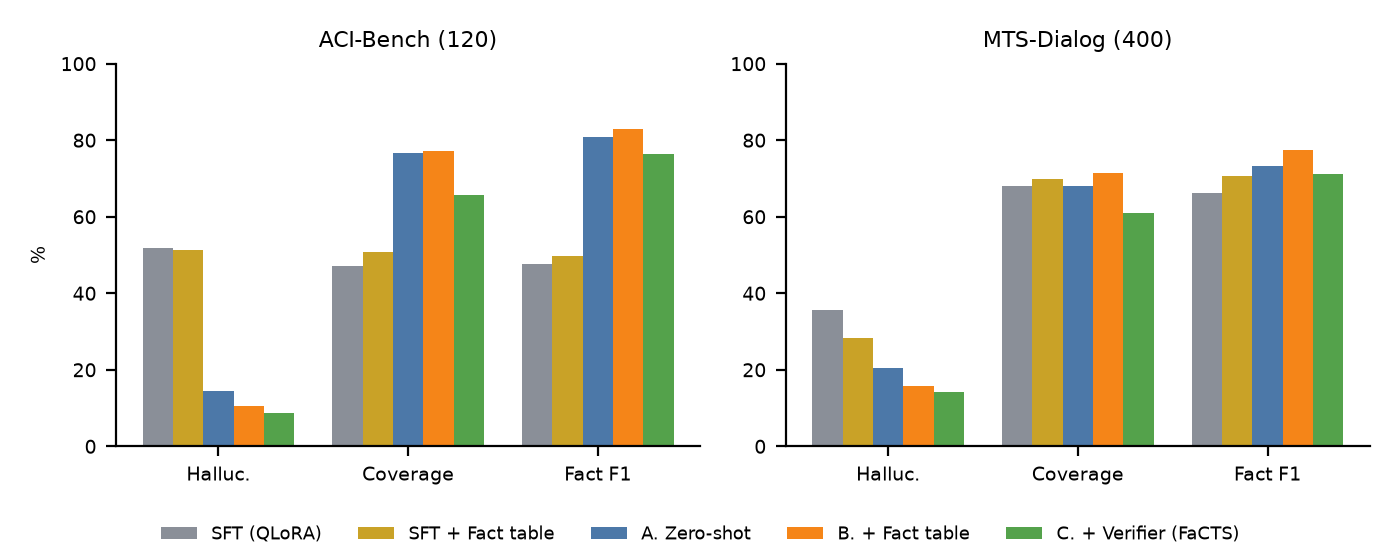
\includegraphics[width=\columnwidth]{figures/factuality.png}
\caption{Hallucination rate, coverage and fact-level F1 per system and dataset (all test items).}\label{fig:fact}
\end{figure}

\begin{table}[t]
\centering
\caption{Paired differences in percentage points (per-item means). $^{*}$: 95\% paired bootstrap interval excludes 0 (10{,}000 resamples).}\label{tab:sig}
\scriptsize
\setlength{\tabcolsep}{2.5pt}
\resizebox{\columnwidth}{!}{\begin{tabular}{@{}llrrrrr@{}}
\toprule
Dataset & Comparison & Halluc. & Neg.\ flip & Num.\ cons. & Coverage & R-L\\
\midrule
ACI-Bench & SFT $-$ A & +37.3$^{*}$ & +9.0$^{*}$ & -26.2$^{*}$ & -29.6$^{*}$ & -14.0$^{*}$\\
ACI-Bench & SFT+F $-$ SFT & -0.6 & +4.0$^{*}$ & +5.5 & +3.5 & -3.1$^{*}$\\
ACI-Bench & B $-$ A & -3.9$^{*}$ & -0.0 & +9.4$^{*}$ & +0.4 & -0.7$^{*}$\\
ACI-Bench & C $-$ B & -1.8$^{*}$ & -0.8 & +0.8 & -11.6$^{*}$ & -1.8$^{*}$\\
\midrule
MTS-Dialog & SFT $-$ A & +14.3$^{*}$ & +1.2 & -5.4$^{*}$ & +0.1 & +9.5$^{*}$\\
MTS-Dialog & SFT+F $-$ SFT & -4.3$^{*}$ & +3.0$^{*}$ & -1.6 & +1.7 & -2.1$^{*}$\\
MTS-Dialog & B $-$ A & -3.5$^{*}$ & +1.2 & -0.7 & +3.6 & -2.7$^{*}$\\
MTS-Dialog & C $-$ B & -0.7 & +0.3 & +2.3$^{*}$ & -10.6$^{*}$ & -0.1\\
\bottomrule
\end{tabular}}
\end{table}


\subsection{Verifier analysis}\label{sec:ver}
The evidence strategy of the verifier was chosen on the validation sets only. Reference sentences of the
120 ACI-Bench and MTS-Dialog validation notes should pass; copies with one injected negation flip or changed
number should fail. With the selected strategy (maximum over whole transcript, top-3 windows and their
union), the verifier passed 72.8\% of 966 reference sentences and caught 60.6\% of 302 corrupted ones (75.4\%
of number changes but only 35.1\% of negation flips), a balanced accuracy of 0.667, against 0.648 for
a single retrieved premise and 0.639 with five windows. Because human references contain some content that
was never said, the pass rate is a lower bound. On the test notes of system B the verifier marked 28.8\% of the
checked sentences red on both datasets (Table~\ref{tab:ver}); no note was emptied. Its weakness on negation
mirrors the finding that general-domain detectors struggle on clinical dialogue~\cite{bn2025fact}.

\begin{table}[t]
\centering
\caption{Verifier verdicts on system B notes (share of checked sentences, \%). Red sentences are dropped.}\label{tab:ver}
\scriptsize
\setlength{\tabcolsep}{3pt}
\resizebox{\columnwidth}{!}{\begin{tabular}{@{}lrrrrrr@{}}
\toprule
Dataset & Notes & Sent. & Green & Yellow & Red & Emptied\\
\midrule
ACI-Bench (120) & 120 & 2905 & 68.0 & 3.2 & 28.8 & 0\\
MTS-Dialog (400) & 400 & 1506 & 69.5 & 1.7 & 28.8 & 0\\
\bottomrule
\end{tabular}}
\end{table}


\subsection{Discussion and limitations}
Three results hold on both datasets with significant paired differences: QLoRA fine-tuning raised
hallucination, the fact table lowered it, and the verifier lowered coverage. Lexical metrics alone would
have ranked the SFT model best on MTS-Dialog, which is why factuality metrics must be reported next to
ROUGE.

The study has limitations. (1) Factuality is measured automatically with our lexicon-based extractor;
human reference notes themselves score 15\% (ACI-Bench) and 28\% (MTS-Dialog) ``hallucination'' under this
metric, which is therefore a floor, not zero, and no clinician evaluation was performed. (2) The SFT
adapter was selected by validation loss on data with few full ACI-Bench notes; a rebalanced adapter might
degenerate less, so its ACI-Bench numbers describe this adapter, not SFT in general. (3) BLEURT and the
deberta-xlarge BERTScore of the shared task were not computed, so only ROUGE is compared with published
systems. (4) MTS-Dialog prompts include the gold section header. (5) All results are from one greedy run.


% =====================================================================================================
\section{Conclusion and Future Work}\label{sec:conc}
We evaluated an open 8B LLM for clinical note generation on the official ACI-Bench and MTS-Dialog test sets
and compared it with published MEDIQA-Chat 2023 systems using the official ROUGE configuration. Untrained
Llama-3.1-8B-Instruct matched GPT-4 zero-shot on both datasets (ROUGE-1 0.519 and 0.303). QLoRA fine-tuning
raised ROUGE on the short MTS-Dialog sections to the level of fine-tuned shared-task systems (0.400), but
increased the entity-level hallucination rate on both datasets (ACI-Bench 14.4\%$\rightarrow$51.7\%,
MTS-Dialog 20.4\%$\rightarrow$35.6\%); adding the fact table to the fine-tuned model did not bring it back
to the level of the untrained model. FaCTS addresses this without training: conditioning the model on a
negation- and dose-aware fact table lowered hallucination to 10.6\% and 15.8\% with no loss of coverage, giving
the best fact-level F1 on both datasets, and sentence-level NLI verification lowered it further to 8.7\% and
14.2\% at a cost of about 11 points of coverage.

Future work follows directly from these results. (1) \emph{Repair instead of drop}: rewrite red sentences
with the generator, as in detector-guided self-refinement~\cite{seethakantha2026hdsr}, to keep their
supported facts. (2) \emph{Factuality preference training}: train an ORPO~\cite{hong2024orpo} adapter on pairs
of reference notes and copies with one injected error (negation flip, dose change, entity swap, inserted
fact), so that the model, not only the pipeline, learns to prefer grounded notes. (3) A better verifier for
dialogue negation, e.g.\ fine-tuning the NLI model on clinical question--answer pairs. (4) Clinician
evaluation of a sample of notes, and the shared-task BERTScore and BLEURT for a complete comparison.
(5) Rebalancing the fine-tuning data towards full notes and selecting checkpoints by factuality rather than
validation loss.


% =====================================================================================================
\begin{thebibliography}{99}
\bibitem{vanveen2024} D.~Van Veen \emph{et al.}, ``Adapted large language models can outperform medical experts in clinical text summarization,'' \emph{Nature Medicine}, vol.~30, pp.~1134--1142, 2024, doi:10.1038/s41591-024-02855-5.
\bibitem{asgari2025} E.~Asgari \emph{et al.}, ``A framework to assess clinical safety and hallucination rates of LLMs for medical text summarisation,'' \emph{npj Digital Medicine}, vol.~8, 2025, doi:10.1038/s41746-025-01670-7.
\bibitem{yim2023aci} W.~Yim \emph{et al.}, ``Aci-bench: a novel ambient clinical intelligence dataset for benchmarking automatic visit note generation,'' \emph{Scientific Data}, vol.~10, 2023, doi:10.1038/s41597-023-02487-3.
\bibitem{abacha2023mts} A.~Ben Abacha, W.~Yim, Y.~Fan, and T.~Lin, ``An empirical study of clinical note generation from doctor-patient encounters,'' in \emph{Proc. EACL}, 2023, pp.~2291--2302, doi:10.18653/v1/2023.eacl-main.168.
\bibitem{abacha2023overview} A.~Ben Abacha, W.~Yim, G.~Adams, N.~Snider, and M.~Yetisgen, ``Overview of the MEDIQA-Chat 2023 shared tasks on the summarization \& generation of doctor-patient conversations,'' in \emph{Proc. 5th Clinical NLP Workshop}, 2023, pp.~503--513, doi:10.18653/v1/2023.clinicalnlp-1.52.
\bibitem{bn2025fact} S.~BN \emph{et al.}, ``Fact-controlled diagnosis of hallucinations in medical text summarization,'' in \emph{Proc. Interspeech}, 2025, doi:10.21437/Interspeech.2025-537.
\bibitem{das2025} A.~B.~Das, S.~Ahmed, and S.~K.~Sakib, ``Hallucinations and key information extraction in medical texts: a comprehensive assessment of open-source large language models,'' in \emph{Proc. IEEE BHI}, 2025, doi:10.1109/BHI67747.2025.11269492.
\bibitem{gekhman2024} Z.~Gekhman \emph{et al.}, ``Does fine-tuning LLMs on new knowledge encourage hallucinations?'' in \emph{Proc. EMNLP}, 2024, pp.~7765--7784, doi:10.18653/v1/2024.emnlp-main.444.
\bibitem{kaplan2026} G.~Kaplan, Z.~Gekhman, Z.~Zhu \emph{et al.}, ``Why fine-tuning encourages hallucinations and how to fix it,'' \emph{arXiv preprint}, 2026.
\bibitem{sharma2023cadence} A.~Sharma, D.~Feldman, and A.~Jain, ``Team Cadence at MEDIQA-Chat 2023: generating, augmenting and summarizing clinical dialogue with large language models,'' in \emph{Proc. 5th Clinical NLP Workshop}, 2023, doi:10.18653/v1/2023.clinicalnlp-1.28.
\bibitem{giorgi2023wanglab} J.~Giorgi, A.~Toma, R.~Xie \emph{et al.}, ``WangLab at MEDIQA-Chat 2023: clinical note generation from doctor-patient conversations using large language models,'' in \emph{Proc. 5th Clinical NLP Workshop}, 2023, doi:10.18653/v1/2023.clinicalnlp-1.36.
\bibitem{lyu2024} M.~Lyu, C.~Peng, X.~Li \emph{et al.}, ``Automatic summarization of doctor-patient encounter dialogues using large language model through prompt tuning,'' \emph{arXiv preprint arXiv:2403.13089}, 2024 (also in AMIA Joint Summits on Translational Science Proc.).
\bibitem{dettmers2023qlora} T.~Dettmers, A.~Pagnoni, A.~Holtzman, and L.~Zettlemoyer, ``QLoRA: efficient finetuning of quantized LLMs,'' in \emph{Advances in NeurIPS 36}, 2023, doi:10.48550/arXiv.2305.14314.
\bibitem{hu2022lora} E.~J.~Hu \emph{et al.}, ``LoRA: low-rank adaptation of large language models,'' in \emph{Proc. ICLR}, 2022, doi:10.48550/arXiv.2106.09685.
\bibitem{laban2022summac} P.~Laban, T.~Schnabel, P.~N.~Bennett, and M.~A.~Hearst, ``SummaC: re-visiting NLI-based models for inconsistency detection in summarization,'' \emph{Trans. ACL}, vol.~10, pp.~163--177, 2022, doi:10.1162/tacl\_a\_00453.
\bibitem{huang2023swing} K.-H.~Huang, S.~Singh, X.~Ma \emph{et al.}, ``SWING: balancing coverage and faithfulness for dialogue summarization,'' in \emph{Findings of EACL}, 2023, doi:10.18653/v1/2023.findings-eacl.37.
\bibitem{seethakantha2026hdsr} S.~K.~Seethakantha, D.~N.~Thai, V.~P.~Gudi \emph{et al.}, ``Hallucination detection-guided preference optimization for clinical summarization,'' \emph{arXiv preprint}, 2026.
\bibitem{dubey2024llama3} A.~Dubey \emph{et al.} (Llama Team, Meta), ``The Llama 3 herd of models,'' \emph{arXiv preprint arXiv:2407.21783}, 2024.
\bibitem{vaswani2017} A.~Vaswani \emph{et al.}, ``Attention is all you need,'' in \emph{Advances in NeurIPS 30}, 2017.
\bibitem{chapman2001negex} W.~W.~Chapman, W.~Bridewell, P.~Hanbury, G.~F.~Cooper, and B.~G.~Buchanan, ``A simple algorithm for identifying negated findings and diseases in discharge summaries,'' \emph{J. Biomedical Informatics}, vol.~34, no.~5, pp.~301--310, 2001, doi:10.1006/jbin.2001.1029.
\bibitem{lv2011bm25plus} Y.~Lv and C.~Zhai, ``Lower-bounding term frequency normalization,'' in \emph{Proc. ACM CIKM}, 2011, pp.~7--16.
\bibitem{he2023debertav3} P.~He, J.~Gao, and W.~Chen, ``DeBERTaV3: improving DeBERTa using ELECTRA-style pre-training with gradient-disentangled embedding sharing,'' in \emph{Proc. ICLR}, 2023.
\bibitem{omi2024soap} Omi Health, ``medical-dialogue-to-soap-summary,'' Hugging Face dataset (synthetic), 2024.
\bibitem{lin2004rouge} C.-Y.~Lin, ``ROUGE: a package for automatic evaluation of summaries,'' in \emph{Text Summarization Branches Out}, ACL Workshop, 2004, pp.~74--81.
\bibitem{zhang2020bertscore} T.~Zhang, V.~Kishore, F.~Wu, K.~Q.~Weinberger, and Y.~Artzi, ``BERTScore: evaluating text generation with BERT,'' in \emph{Proc. ICLR}, 2020.
\bibitem{hong2024orpo} J.~Hong, N.~Lee, and J.~Thorne, ``ORPO: monolithic preference optimization without reference model,'' in \emph{Proc. EMNLP}, 2024, doi:10.48550/arXiv.2403.07691.
\end{thebibliography}

\end{document}
